\documentclass[letterpaper]{article}
\usepackage{underscore}
\usepackage[left=2.0cm, right=2.0cm, top=2.0cm]{geometry}
\usepackage[utf8]{inputenc}
\usepackage{graphicx}
\usepackage{graphics}
\usepackage[spanish]{babel}
\usepackage{lipsum}
\usepackage{float}
\usepackage{subfigure}
\title{EV\_2\_3\_Explicar\_arreglos\_y\_parametros\_de\_los\_amplificadores\_clase\_B}
\author{Ledesma Hernández Miguel Ángel}
\date{01/oct/2019}

\begin{document}
\maketitle
\begin{large}
\begin{center}
\vspace{13cm}
4-A Mecatrónica\\

Universidad Politécnica de la Zona Metropolitana de Guadalajara

\end{center}



\newpage
Cuando hablamos de amplificadores clase 'B' debemos hablar de los amplificadores en general, sobre todo de los amplificadores clase 'A'.\\
La logística de este tipo de amplificador podria traducirce a; si el amplificador clase 'A' solo puede amplificar la almentación que se tiene, ¿Qué efecto tendría si se ponen dos transistores?, es decir que en esta clase de amplificador tenemos dos transistores que trabajan a la par, y cada uno de ellos lleva una parte de la carga del trabajo, uno no carga con todo, si no que los dos cargan con el trabajo. Como una analogía podriamos usar una góndola; en vez de que reme una sola persona, remarán dos y ésta irá más rápido.\\
Éste amplificador lleva dos transistores y tambien se le conoce como "\textbf{PushPull}" y comunmente los podemos encontrar como el siguiente diagrama \\
\textbf{Nota importante: Ambos transistores deben ser iguales}\\
\begin{figure}[hbtp]
\centering
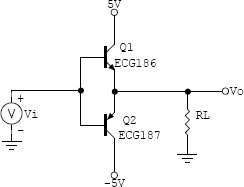
\includegraphics[scale=1]{Imagenes/img1.jpg}
\caption{Circuito}
\end{figure}\\
Cuando los transistores son cumplidos, es decir uno toma 0.6 o 0.7 v en la parte de base funciona y es entonces cuando el voltaje pasa de forma que la señal entra y es amplificada dentrod e los transistores Q1 y cuando se cumple, también es amplificada en Q2, esto va a la carga que va despues de los dos transistores, la tierra debajo de RL, puede ser una bocina, audifono...\\

Mientras una cumple el semiciclo, la otra amplifica de manera inversa el semiciclo, dejando una onda amplificada de mismas proporciones relativas con respecto a la onda original.

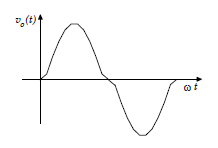
\includegraphics[scale=1]{Imagenes/onda.png} 
\\
nota: este no amplificará amenos que los transistores reciban una señal de 0.6 o 0.7 V en su común, si no lo reciben no podrán amplificar y a esto se le llamará distorsión.\\

Decimos, este amplificador no tiene utilidad como tal. Pues no, esta distorsión es casi imperceptible cuando trabajamos con altos voltajes. Por ejemplo cuando es a 50V.\\
\textbf{Bibliografías:}

Website title: 	146.83.206.1\\
URL: 	http://146.83.206.1/~jhuircan/PDF_CTOI/AP01a.pdf


\end{large}
\end{document}